\documentclass[border=10pt]{standalone}
\usepackage[svgnames]{xcolor}
\usepackage{amsmath}
\usepackage{pgfplots}
\pgfplotsset{compat=newest}
\usepackage[sfdefault]{FiraSans}
\usepackage{FiraMono}
\renewcommand*\familydefault{\sfdefault}
\begin{document}
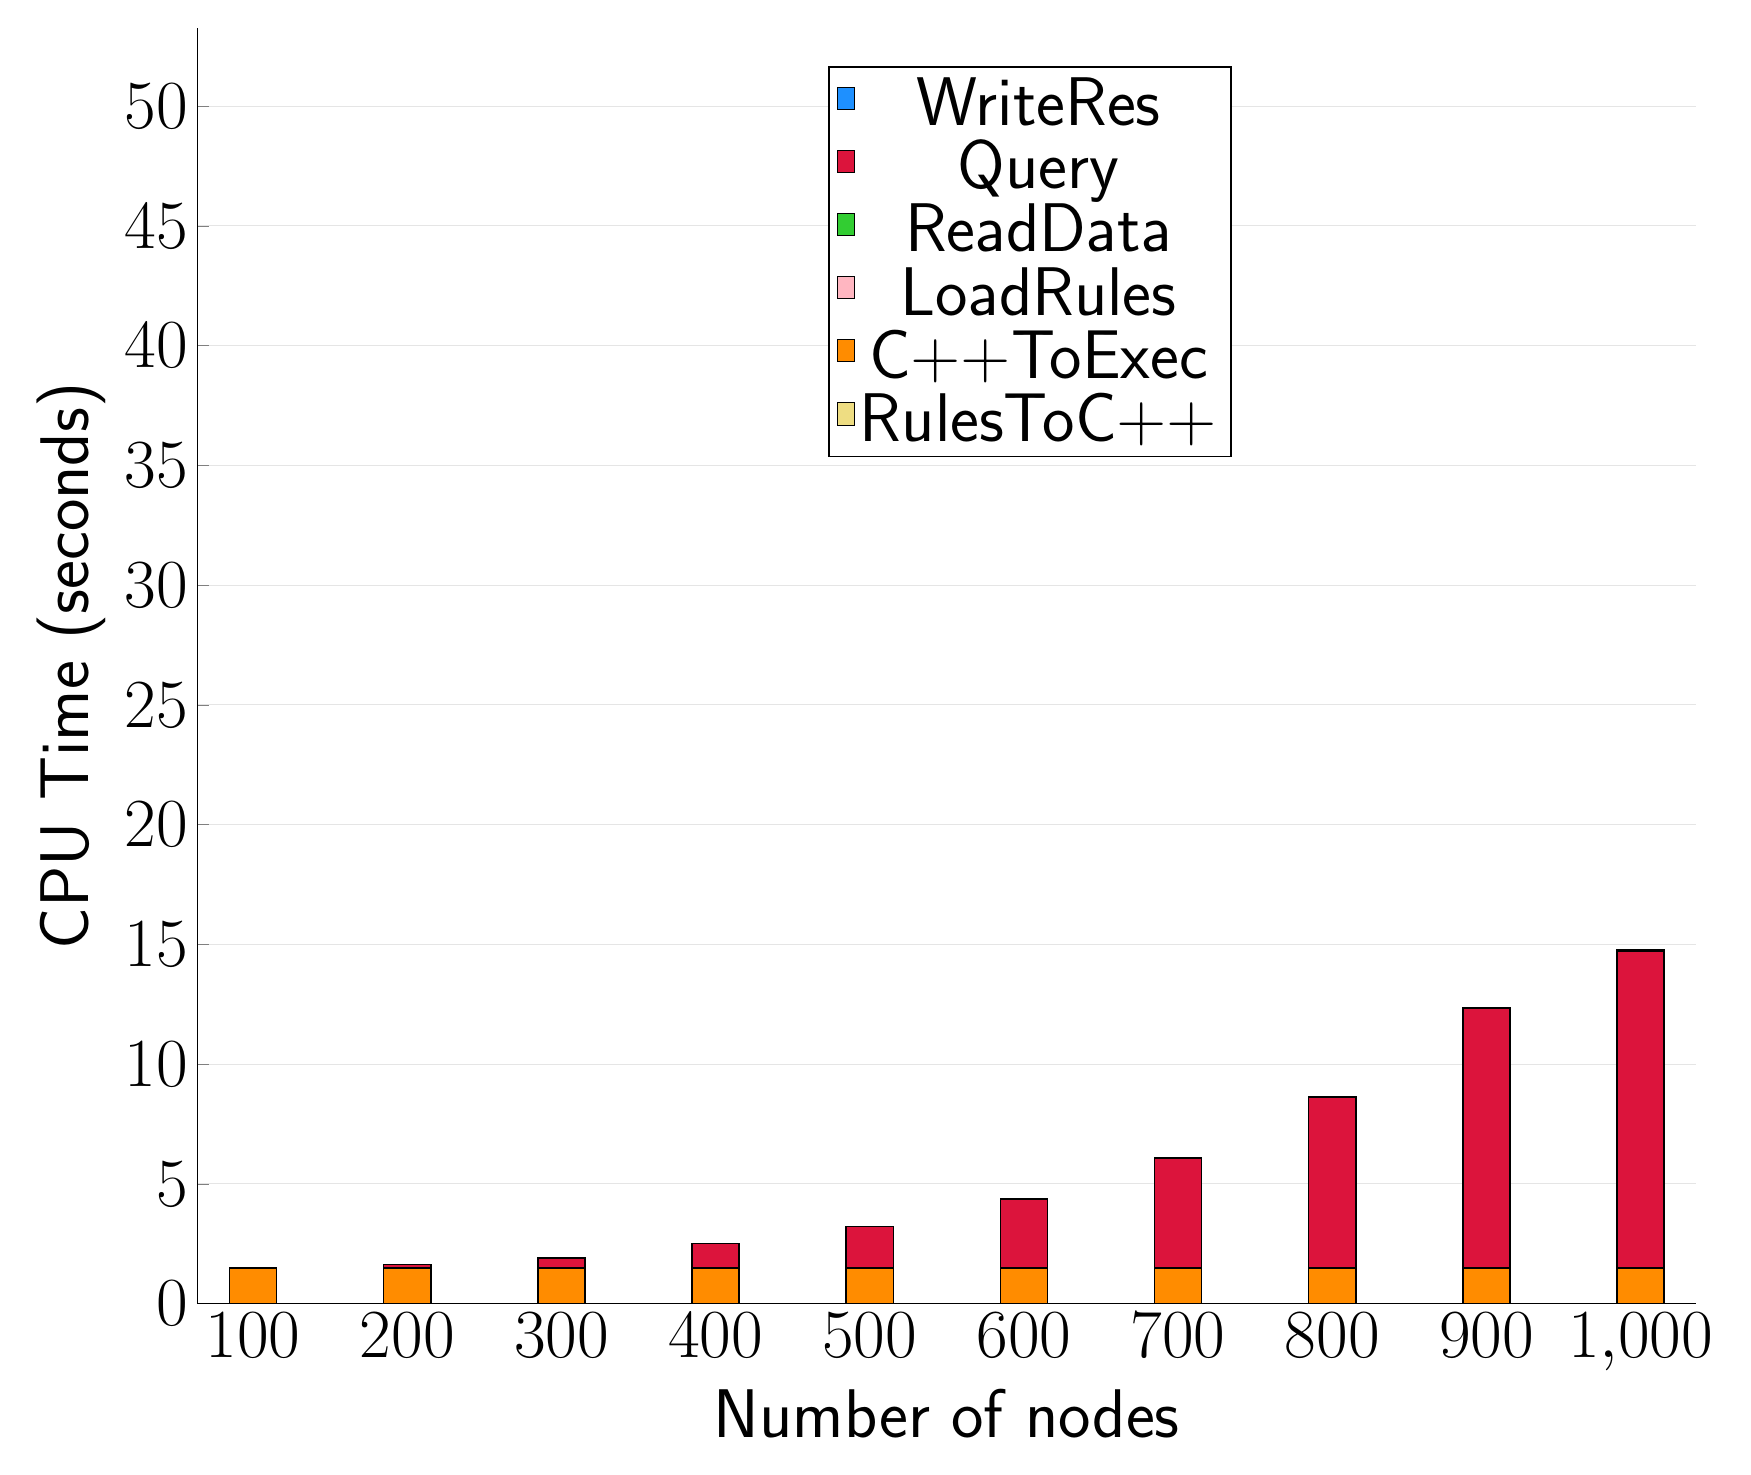
\begin{tikzpicture}
\begin{axis}[
   ybar stacked,
   width=1.7\textwidth,
   bar width=0.6cm,
   ymajorgrids, tick align=inside,
   major grid style={draw=gray!20},
   xtick=data,
   ymin=0, ymax=53.25004,
   axis x line*=bottom,
   axis y line*=left,
   enlarge x limits=0.04,
   legend style={
       at={(0.69, 0.97)},
       anchor=north east,
       legend columns=1,
       font=\Huge,
   },
   ylabel={CPU Time (seconds)},
   xlabel={Number of nodes},
   label style={font=\Huge},
   tick label style={font=\Huge},
]
\addlegendimage{fill=DodgerBlue, draw=black, line width=0.2pt}
\addlegendentry{WriteRes}
\addlegendimage{fill=Crimson, draw=black, line width=0.2pt}
\addlegendentry{Query}
\addlegendimage{fill=LimeGreen, draw=black, line width=0.2pt}
\addlegendentry{ReadData}
\addlegendimage{fill=LightPink, draw=black, line width=0.2pt}
\addlegendentry{LoadRules}
\addlegendimage{fill=DarkOrange, draw=black, line width=0.2pt}
\addlegendentry{C++ToExec}
\addlegendimage{fill=LightGoldenrod, draw=black, line width=0.2pt}
\addlegendentry{RulesToC++}
\addplot +[fill=LightGoldenrod, draw=black, line width=0.55pt] coordinates {
(100, 0.006000000000000001)
(200, 0.006000000000000001)
(300, 0.006000000000000001)
(400, 0.004000000000000001)
(500, 0.006000000000000001)
(600, 0.004000000000000001)
(700, 0.0020000000000000005)
(800, 0.004000000000000001)
(900, 0.004000000000000001)
(1000, 0.0020000000000000005)
};
\addplot +[fill=DarkOrange, draw=black, line width=0.55pt] coordinates {
(100, 1.47)
(200, 1.47)
(300, 1.4739999999999998)
(400, 1.4739999999999998)
(500, 1.472)
(600, 1.472)
(700, 1.4780000000000002)
(800, 1.4700000000000002)
(900, 1.478)
(1000, 1.472)
};
\addplot +[fill=LightPink, draw=black, line width=0.55pt] coordinates {
(100, 0.00018619999999999997)
(200, 0.0001898)
(300, 0.0002)
(400, 0.00018419999999999998)
(500, 0.00018600000000000002)
(600, 0.0001862)
(700, 0.0001912)
(800, 0.0001876)
(900, 0.00018419999999999998)
(1000, 0.00018779999999999998)
};
\addplot +[fill=LimeGreen, draw=black, line width=0.55pt] coordinates {
(100, 0.0010528)
(200, 0.0018574)
(300, 0.0025691999999999998)
(400, 0.0033444)
(500, 0.0039109999999999995)
(600, 0.0043733999999999995)
(700, 0.0051383999999999996)
(800, 0.0056234)
(900, 0.0068032)
(1000, 0.0071346000000000005)
};
\addplot +[fill=Crimson, draw=black, line width=0.55pt] coordinates {
(100, 0.0357756)
(200, 0.14762720000000001)
(300, 0.41334040000000005)
(400, 1.0184260000000003)
(500, 1.7314640000000001)
(600, 2.857268)
(700, 4.564864)
(800, 7.119124000000001)
(900, 10.834079999999998)
(1000, 13.250040000000002)
};
\addplot +[fill=DodgerBlue, draw=black, line width=0.55pt] coordinates {
(100, 0.0011227999999999998)
(200, 0.0026436000000000003)
(300, 0.0052868)
(400, 0.009715000000000001)
(500, 0.0141508)
(600, 0.019548799999999998)
(700, 0.0267154)
(800, 0.0355072)
(900, 0.0465994)
(1000, 0.052561000000000004)
};
\end{axis}
\end{tikzpicture}

\end{document}
